\documentclass[12pt,letterpaper]{article}
\usepackage[utf8]{inputenc}
\usepackage[spanish]{babel}
\usepackage{graphicx}
\usepackage[left=2cm,right=2cm,top=2cm,bottom=2cm]{geometry}
\usepackage{graphicx} % figuras
% \usepackage{subfigure} % subfiguras
\usepackage{float} % para usar [H]
\usepackage{amsmath}
%\usepackage{txfonts}
\usepackage{stackrel} 
\usepackage{multirow}
\usepackage{enumerate} % enumerados
\renewcommand{\labelitemi}{$-$}
\renewcommand{\labelitemii}{$\cdot$}
% \author{}
% \title{Caratula}
\begin{document}

% Fancy Header and Footer
% \usepackage{fancyhdr}
% \pagestyle{fancy}
% \cfoot{}
% \rfoot{\thepage}
%

% \usepackage[hidelinks]{hyperref} % CREA HYPERVINCULOS EN INDICE

% \author{}
\title{Caratula}

\begin{titlepage}
\begin{center}
\large{UNIVERSIDAD PRIVADA DE TACNA}\\
\vspace*{-0.025in}
\begin{figure}[htb]
\begin{center}

\includegraphics[width=7cm]{./images/logo}
\end{center}
\end{figure}
\vspace*{0.15in}
INGENIERIA DE SISTEMAS  \\

\vspace*{0.3in}
\begin{large}
\textbf{TITULO:} \\
\end{large}

\vspace*{0.1in}
\begin{Large}
\textbf{Informe de Laboratorio 03: Creando un Cubo Multimensional con SQL Server Analysis Services} \\

\end{Large}

\vspace*{0.3in}
\begin{Large}
\textbf{CURSO:} \\
\end{Large}

\vspace*{0.1in}
\begin{large}
INTELIGENCIA DE NEGOCIOS\\
\end{large}

\vspace*{0.3in}
\begin{Large}
\textbf{DOCENTE:} \\
\end{Large}

\vspace*{0.1in}
\begin{large}
 Ing. Patrick Cuadros Quiroga\\
\end{large}

\vspace*{0.4in}
\vspace*{0.1in}
\begin{large}
\textbf{INTEGRANTES:} \\
\begin{flushleft}
Willian Huillca Umpiri \hfill	(2015053793)\\

\centering  %CENTRA UN TEXTO
\vspace*{0.9in}
\begin{large}
TACNA-PERU\\ 
2020\\
\end{large}

\end{flushleft}
\end{large}
\end{center}

\end{titlepage}


\tableofcontents % INDICE
\thispagestyle{empty} % INDICE SIN NUMERO
\newpage
\setcounter{page}{1} % REINICIAR CONTADOR DE PAGINAS DESPUES DEL INDICE


\section{Procedimiento} 

Primeramente crearemos una base de datos llamada BDTEST.Abrir el SQL Server Data Tools y dirigirnos a la pestaña de Business Intelligence -> Analysis Services. Como se creará un Modelo Multidimensional desde 0 , seleccionaremos la primera opción. En la casilla de Name le colocamos un nombre al proyecto y a la solución:
	\begin{center}
	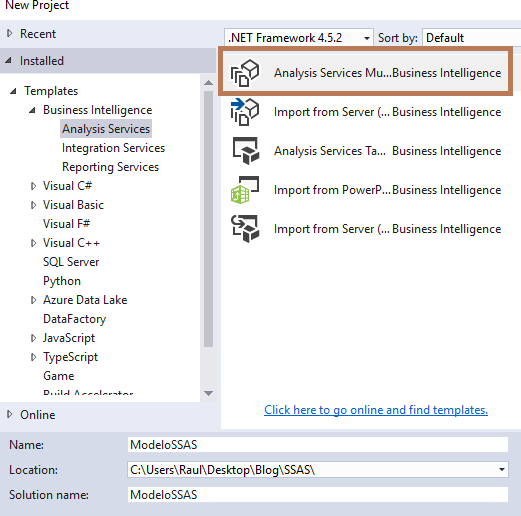
\includegraphics[width=\columnwidth]{images/task1/1}
	\end{center}	

\section{ACTIVIDAD 01 Creación de un Data Source}

En el Solution Explorer nos ubicamos en Data Sources y click derecho, seleccionando la opción de New Data Source
	\begin{center}
	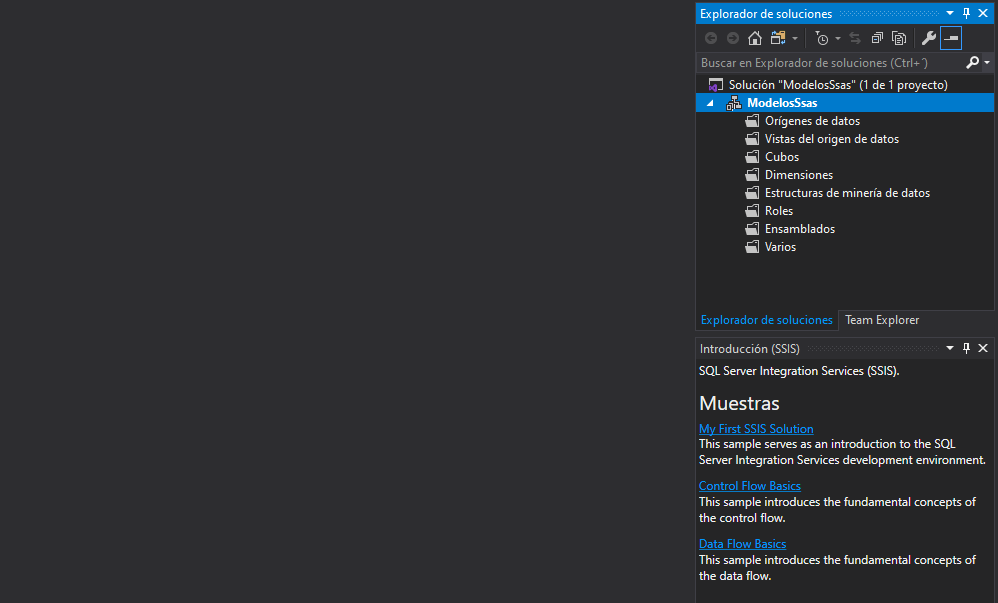
\includegraphics[width=\columnwidth]{images/task1/2}
	\end{center}	

Se nos abrirá una ventana de resumen. Click en Next:
	\begin{center}
	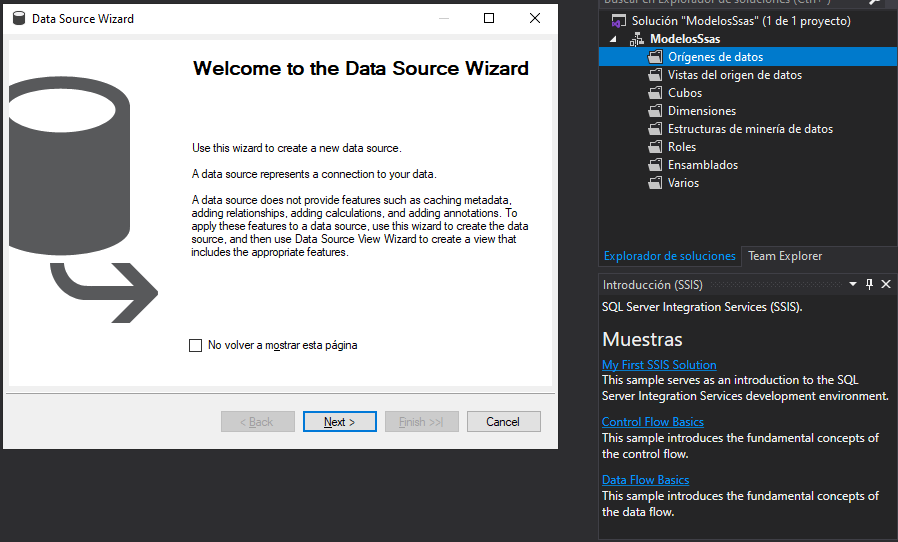
\includegraphics[width=\columnwidth]{images/task1/3}
	\end{center}	

Colocamos el nombre del Server donde se ubica la base de datos, en mi caso como es local coloco “.” , indicándole que es localhost. Ingresamos las credenciales y la base de datos Adventure Works DW 2014. Luego Click en Ok:
	\begin{center}
	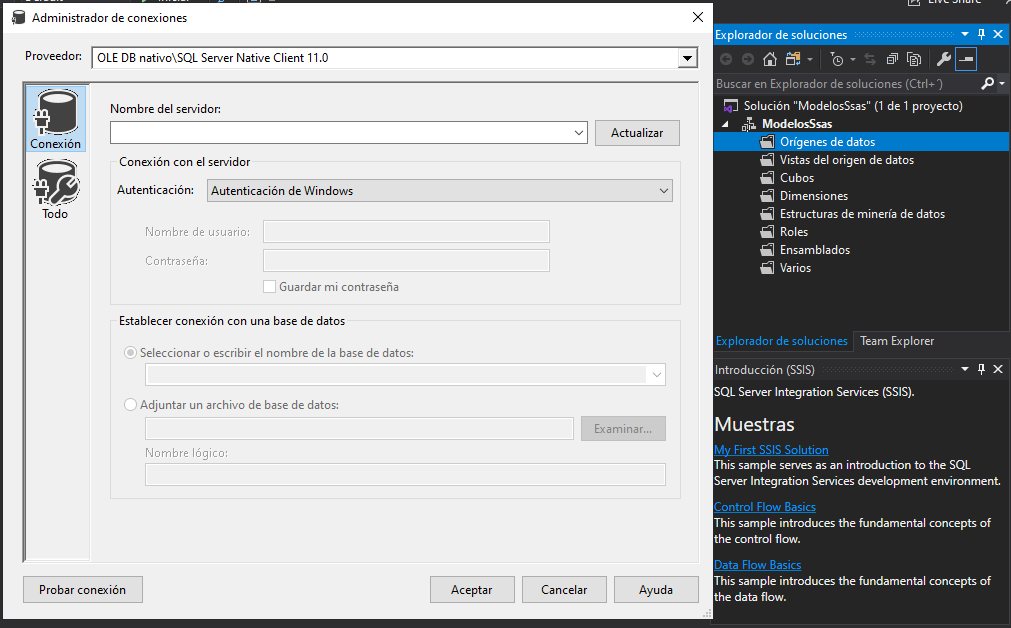
\includegraphics[width=\columnwidth]{images/task1/4}
    \end{center}	
    
Si todo está bien nos aparecerá la conexión creada en la sección de Data connections:
	\begin{center}
	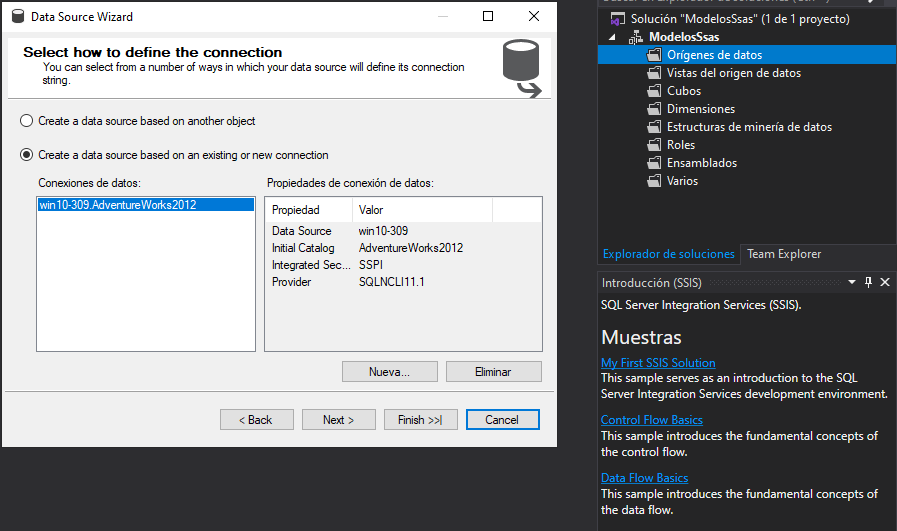
\includegraphics[width=\columnwidth]{images/task1/5}
    \end{center}	
    
En la ventana siguiente podemos definir las credenciales del Analysis Services y que utilizará para conectarse al Data Source. En este caso utilizaremos las mismas credenciales del servicio. Para eso elegimos Use the service account:
	\begin{center}
	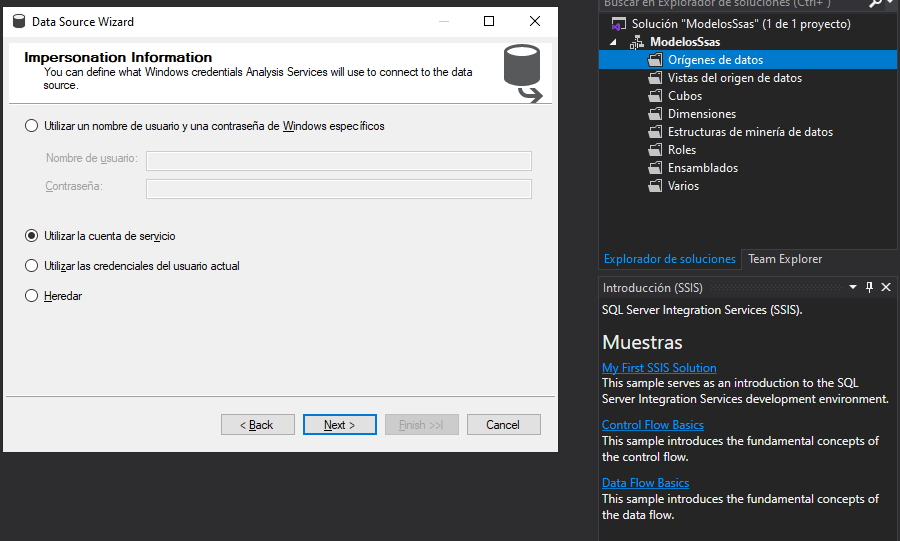
\includegraphics[width=\columnwidth]{images/task1/6}
    \end{center}	
    
	\begin{center}
	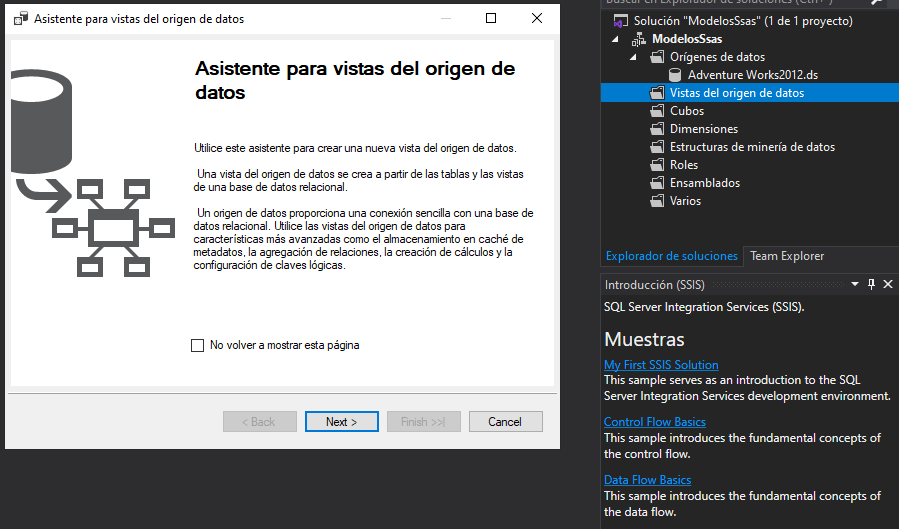
\includegraphics[width=\columnwidth]{images/task1/7}
    \end{center}	
Colocamos un nombre para el Data Source y click en Finish:
	\begin{center}
	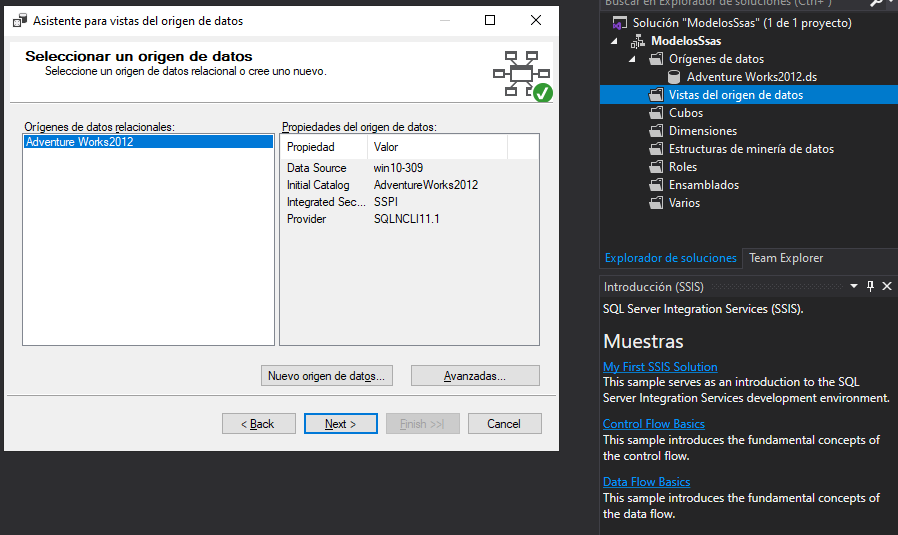
\includegraphics[width=\columnwidth]{images/task1/8}
    \end{center}	

\section{ACTIVIDAD 02 Creación de un Data Source View}

Si bien es cierto hemos creado una conexión hacia Adventure Works DW, solo trabajaremos con algunas tablas. 			Seleccionamos las tablas DimDate,DimProduct y FactInternetSales:
	\begin{center}
	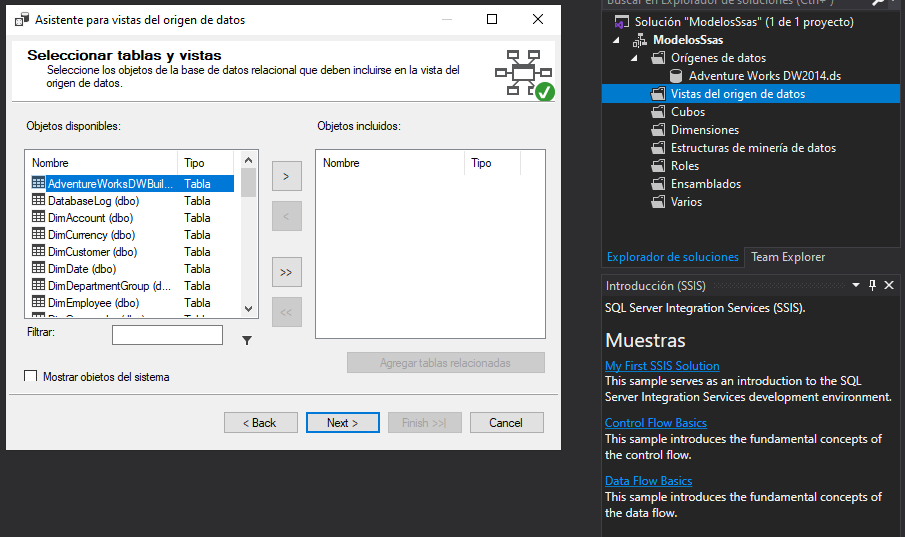
\includegraphics[width=\columnwidth]{images/task1/9}
    \end{center}	
    
Colocamos un nombre el Data Source View creado y click en Finish:
	\begin{center}
	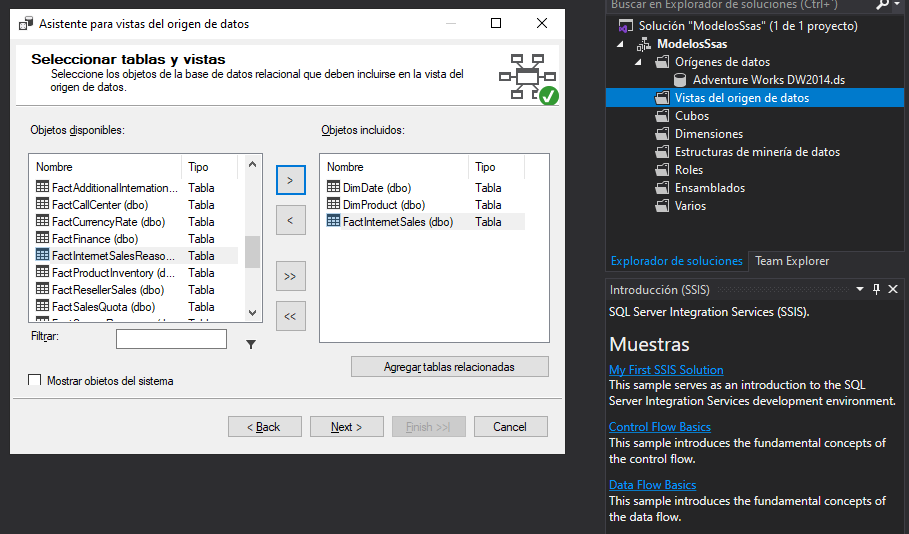
\includegraphics[width=\columnwidth]{images/task1/10}
    \end{center}	
    
	\begin{center}
	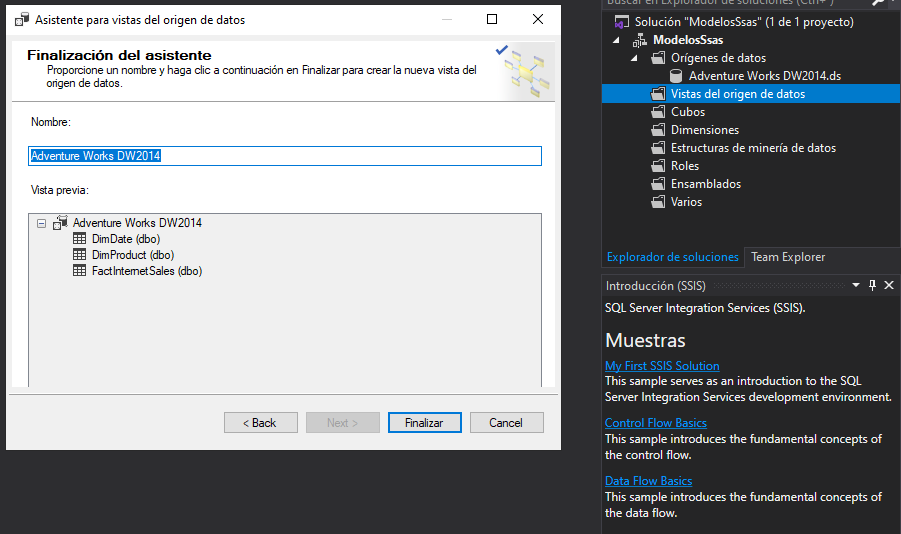
\includegraphics[width=\columnwidth]{images/task1/11}
    \end{center}	
    
Si todo va bien visualizaremos las tablas seleccionadas en el Data Source View:
	\begin{center}
	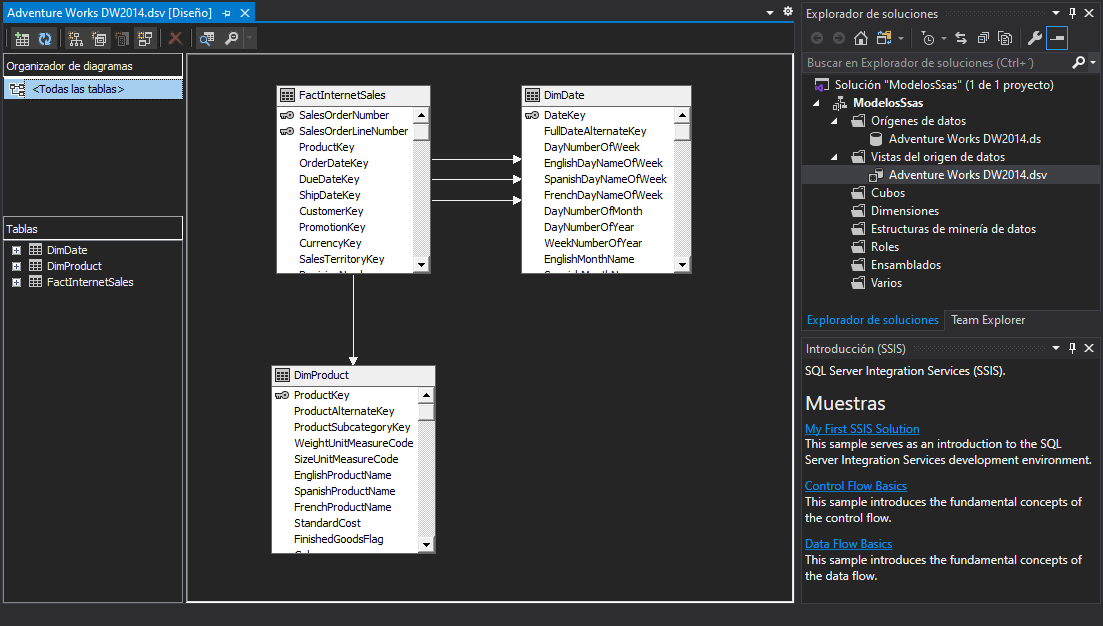
\includegraphics[width=\columnwidth]{images/task1/12}
	\end{center}	
	
\section{ACTIVIDAD 03 Creación de un Cubo}

En el Solution Explorer nos ubicamos en Cubes y click derecho, seleccionando la opción de New Cube
	\begin{center}
	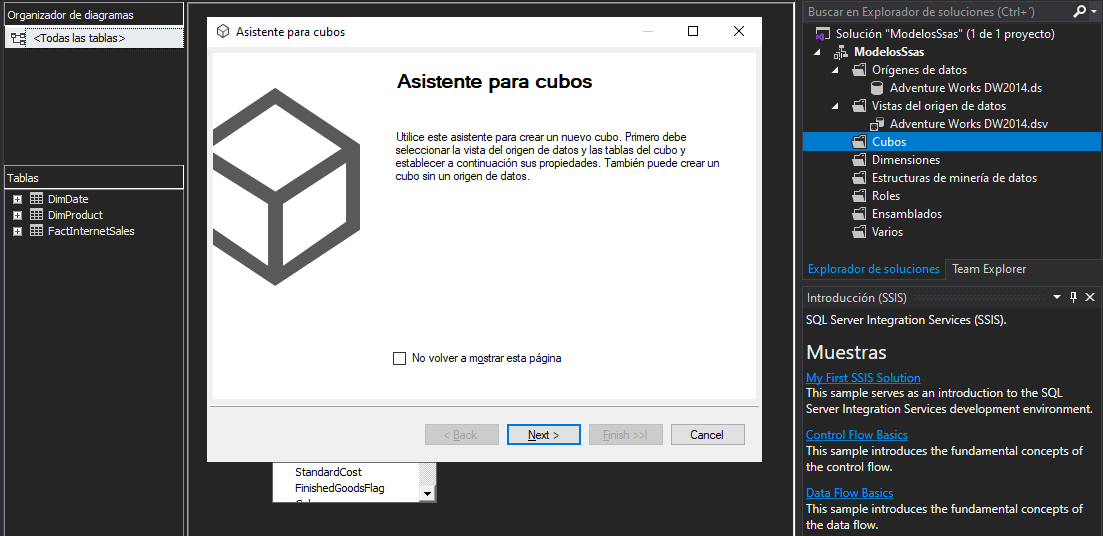
\includegraphics[width=\columnwidth]{images/task1/13}
    \end{center}	
    
Aquí seleccionaremos la FactTable (Tablas de Hechos) , en este caso ubicamos FactInternetSales
	\begin{center}
	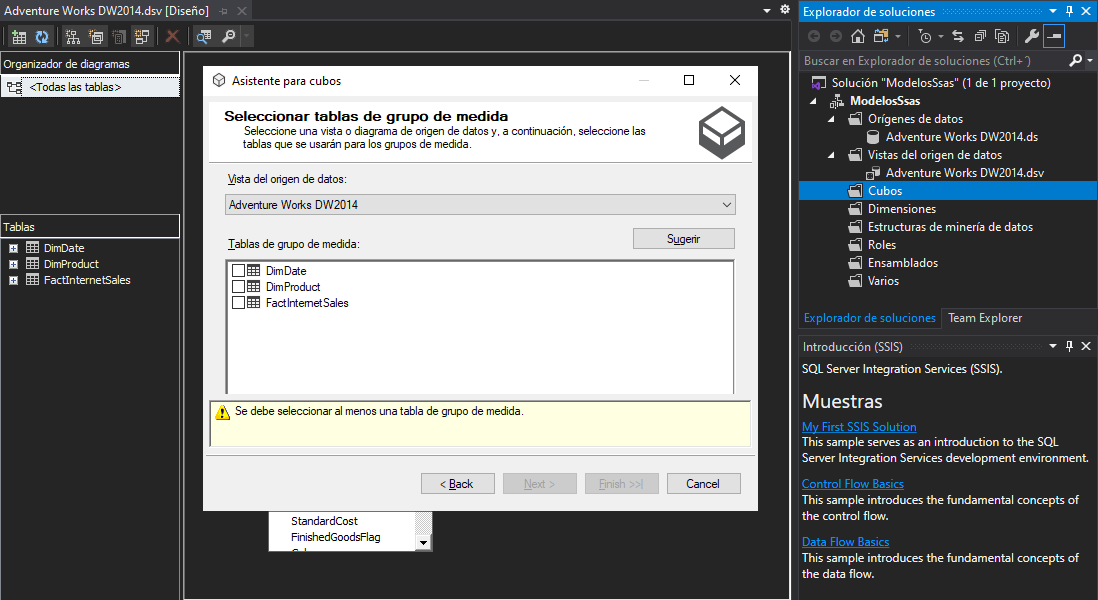
\includegraphics[width=\columnwidth]{images/task1/14}
    \end{center}	
    
Automáticamente el Data Tools identificará todos los campos numéricos y los marcará como candidatos a ser medidas. Podemos observar que inclusive marca los campos utilizados como Foregin Keys. En este caso, seleccionamos solo Order Quantity y Sales Amount:
	\begin{center}
	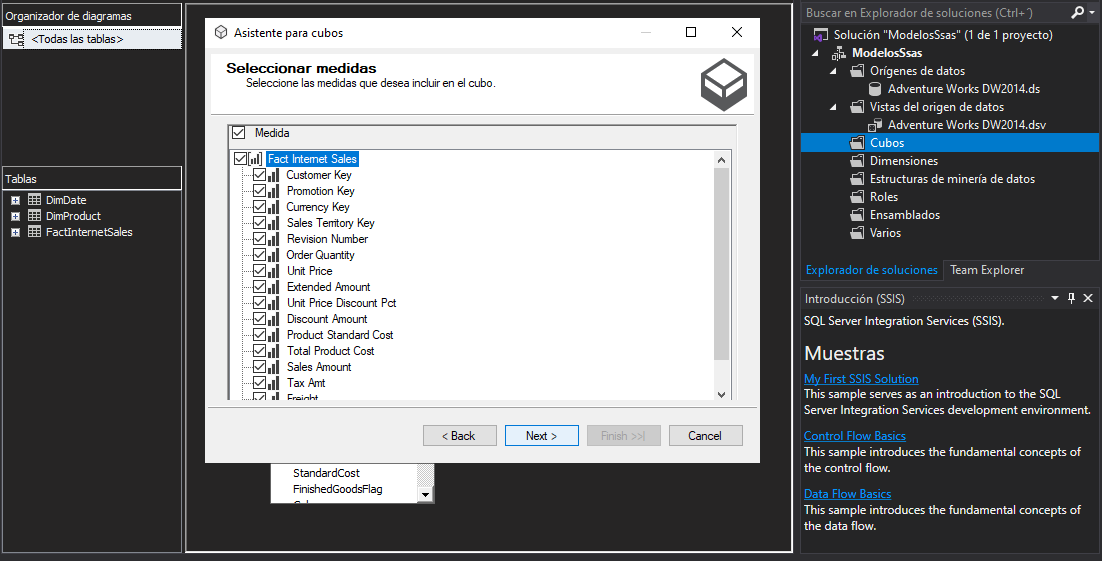
\includegraphics[width=\columnwidth]{images/task1/15}
    \end{center}	
    
Aquí seleccionamos las dimensiones por las cuales será analizada la data. Inclusive el Data Tools te indica que podría tomar la misma FactTable como Dimensión. Seleccionamos Dim Date y Dim Product:
	\begin{center}
	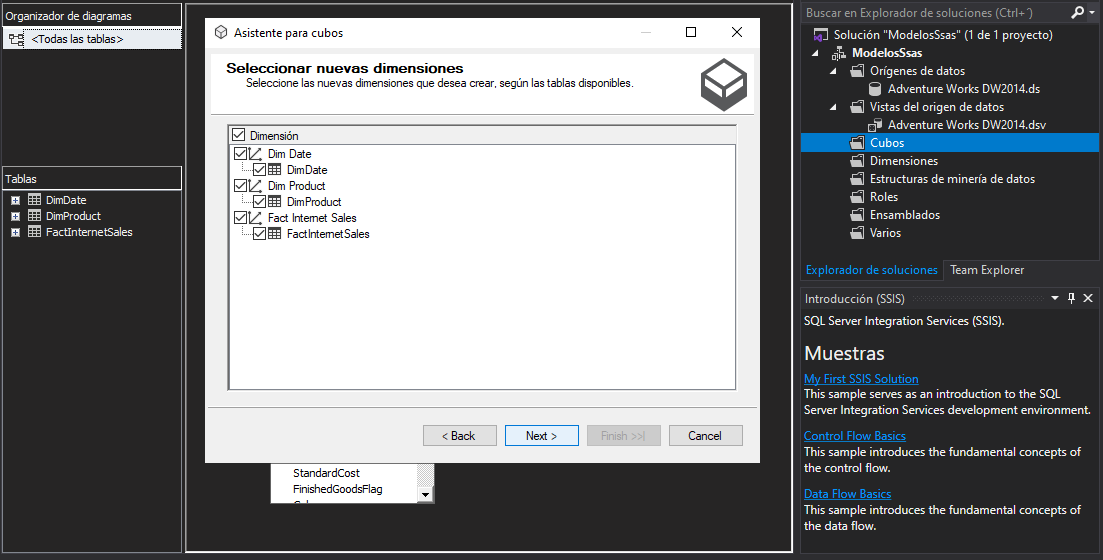
\includegraphics[width=\columnwidth]{images/task1/16}
	\end{center}	

Colocamos un nombre el cubo:
	\begin{center}
	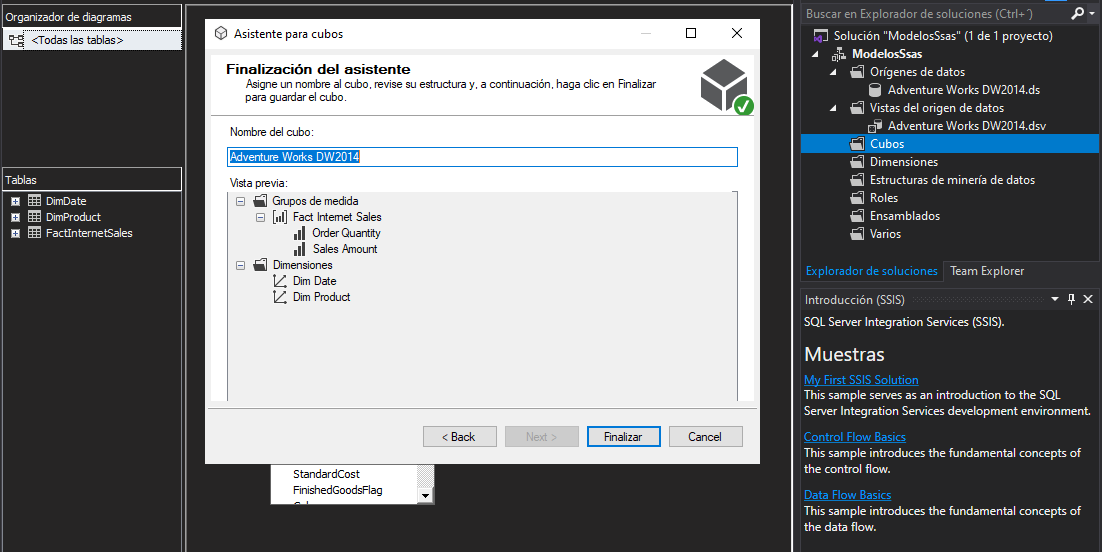
\includegraphics[width=\columnwidth]{images/task1/17}
	\end{center}	
	
En el Solution Explorer nos ubicamos en el nuevo cubo creado CubeSales y click derecho, seleccionando la opción de Process
		\begin{center}
	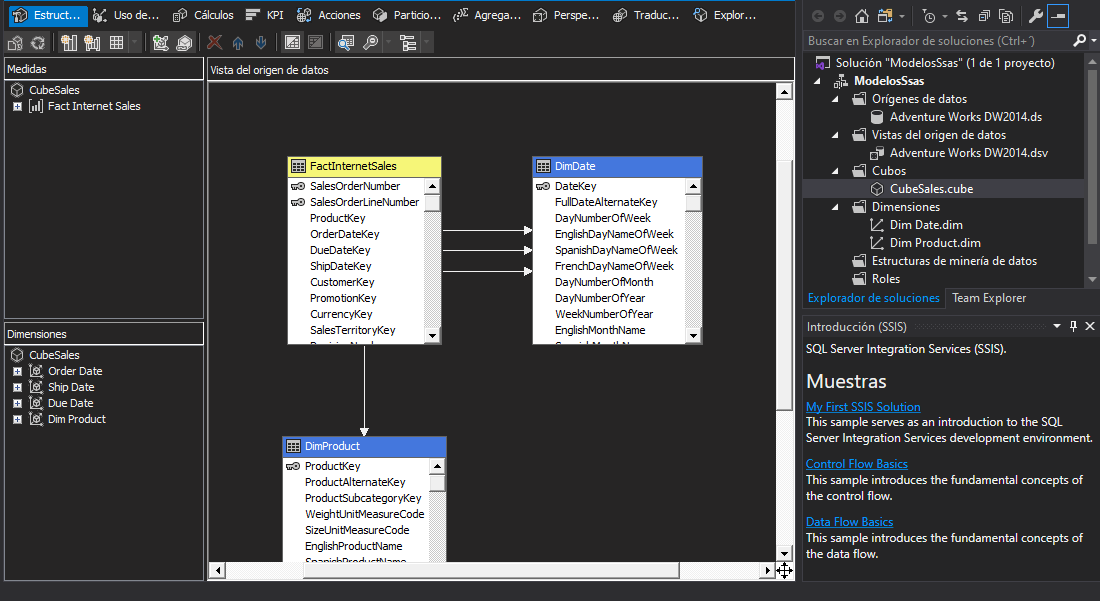
\includegraphics[width=\columnwidth]{images/task1/18}
	\end{center}	
	

	

\include{sections/Task03}
\end{document}